\documentclass[a4paper,11pt]{book}
%\documentclass[a4paper,twoside,11pt,titlepage]{book}
\usepackage{listings}
\usepackage[utf8]{inputenc}
\usepackage[spanish]{babel}

% \usepackage[style=list, number=none]{glossary} %
%\usepackage{titlesec}
%\usepackage{pailatino}

\usepackage[
backend=biber,
style=alphabetic,
sorting=ynt
]{biblatex}
\addbibresource{bibliografia.bib}

\usepackage{breakcites}
\usepackage{float}

\decimalpoint
\usepackage{dcolumn}
\newcolumntype{.}{D{.}{\esperiod}{-1}}
\makeatletter
\addto\shorthandsspanish{\let\esperiod\es@period@code}
\makeatother


%\usepackage[chapter]{algorithm}
\RequirePackage{verbatim}
%\RequirePackage[Glenn]{fncychap}
\usepackage{fancyhdr}
\usepackage{graphicx}
\graphicspath{{./imagenes}}
\usepackage{afterpage}

\usepackage{tikz}
\usetikzlibrary{arrows.meta, positioning}
\usepackage{float}

\usepackage{longtable}

\usepackage[pdfborder={000}]{hyperref} %referencia

% ********************************************************************
% Re-usable information
% ********************************************************************
\newcommand{\myTitle}{Aplicación de renderizado 3D\xspace}
\newcommand{\myDegree}{Grado en ingeniería informática\xspace}
\newcommand{\myName}{Pablo Cantudo Gómez\xspace}
\newcommand{\myProf}{Juan Carlos Torres Cantero y Luis López Escudero\xspace}
%\newcommand{\mySupervisor}{Put name here\xspace}
\newcommand{\myFaculty}{Escuela Técnica Superior de Ingenierías Informática y de
Telecomunicación\xspace}
\newcommand{\myFacultyShort}{E.T.S. de Ingenierías Informática y de
Telecomunicación\xspace}
\newcommand{\myDepartment}{Departamento de Lenguajes y Sistemas Informáticos\xspace}
\newcommand{\myUni}{\protect{Universidad de Granada}\xspace}
\newcommand{\myLocation}{Granada\xspace}
\newcommand{\myTime}{\today\xspace}
\newcommand{\myVersion}{Version 0.1\xspace}


\usepackage{dirtree}
\usepackage{url}
\usepackage{colortbl,longtable}
\usepackage[stable]{footmisc}
\usepackage{index}

\makeindex
\usepackage[toc,nonumberlist]{glossaries}
\makeglossaries

% Definición de comandos que me son tiles:
%\renewcommand{\indexname}{Índice alfabético}
%\renewcommand{\glossaryname}{Glosario}

\pagestyle{fancy}
\fancyhf{}
\fancyhead[LO]{\leftmark}
\fancyhead[RE]{\rightmark}
\fancyhead[RO,LE]{\textbf{\thepage}}
\renewcommand{\chaptermark}[1]{\markboth{\textbf{#1}}{}}
\renewcommand{\sectionmark}[1]{\markright{\textbf{\thesection. #1}}}

\setlength{\headheight}{1.5\headheight}

\newcommand{\HRule}{\rule{\linewidth}{0.5mm}}
%Definimos los tipos teorema, ejemplo y definición podremos usar estos tipos
%simplemente poniendo \begin{teorema} \end{teorema} ...
\newtheorem{teorema}{Teorema}[chapter]
\newtheorem{ejemplo}{Ejemplo}[chapter]
\newtheorem{definicion}{Definición}[chapter]

\definecolor{gray97}{gray}{.97}
\definecolor{gray75}{gray}{.75}
\definecolor{gray45}{gray}{.45}
\definecolor{gray30}{gray}{.94}

\definecolor{codegreen}{rgb}{0,0.6,0}
\definecolor{codegray}{rgb}{0.5,0.5,0.5}
\definecolor{codepurple}{rgb}{0.58,0,0.82}
\definecolor{backcolour}{rgb}{0.95,0.95,0.92}

\usepackage{xcolor}

\lstset{
   backgroundcolor=\color{backcolour},   
   commentstyle=\color{codegreen},
   keywordstyle=\color{magenta},
   numberstyle=\tiny\color{codegray},
   stringstyle=\color{codepurple},
   basicstyle=\ttfamily\footnotesize,
   breakatwhitespace=false,         
   breaklines=true,                 
   captionpos=b,                    
   keepspaces=true,                 
   numbers=left,                    
   numbersep=5pt,                  
   showspaces=false,                
   showstringspaces=false,
   showtabs=false,                  
   tabsize=2
}
 
% minimizar fragmentado de listados
\lstnewenvironment{listing}[1][]
   {\lstset{#1}\pagebreak[0]}{\pagebreak[0]}

\lstdefinestyle{CodigoC}
   {
	basicstyle=\scriptsize,
	frame=single,
	language=C,
	numbers=left
   }
\lstdefinestyle{python}
   {
	basicstyle=\small,
	frame=single,
	backgroundcolor=\color{gray30},
	language=C++,
	numbers=left
   }

 
\lstdefinestyle{Consola}
   {basicstyle=\scriptsize\bf\ttfamily,
    backgroundcolor=\color{gray30},
    frame=single,
    numbers=none
   }


\newcommand{\bigrule}{\titlerule[0.5mm]}


%Para conseguir que en las páginas en blanco no ponga cabecerass
\makeatletter
\def\clearpage{%
  \ifvmode
    \ifnum \@dbltopnum =\m@ne
      \ifdim \pagetotal <\topskip
        \hbox{}
      \fi
    \fi
  \fi
  \newpage
  \thispagestyle{empty}
  \write\m@ne{}
  \vbox{}
  \penalty -\@Mi
}
\makeatother

\usepackage{pdfpages}
\begin{document}
\begin{titlepage}
 
 
\newlength{\centeroffset}
\setlength{\centeroffset}{-0.5\oddsidemargin}
\addtolength{\centeroffset}{0.5\evensidemargin}
\thispagestyle{empty}

\noindent\hspace*{\centeroffset}\begin{minipage}{\textwidth}

\centering

\includegraphics[width=0.9\textwidth]{imagenes/logo.png}\\[1.4cm]

\textsc{ \Large TRABAJO FIN DE GRADO\\[0.2cm]}
\textsc{ GRADO EN INGENIERÍA INFORMÁTICA}\\[1cm]
% Upper part of the page
% 
% Title
{\Huge\bfseries \\ Desarrollo de una aplicaci´on
de modelado 3D}
\noindent\rule[-1ex]{\textwidth}{3pt}\\[3.5ex]
{\large\bfseries Motor de renderizado en tiempo real basada en SDFs}
\end{minipage}

\vspace{2.5cm}
\noindent\hspace*{\centeroffset}\begin{minipage}{\textwidth}
\centering

\textbf{Autor}\\ {Pablo Cantudo Gómez}\\[2.5ex]
\textbf{Directores}\\
{Juan Carlos Torres Cantero y Luis López Escudero\\}\\[2cm]

\includegraphics[width=0.3\textwidth]{imagenes/etsiit_logo.png}\\[0.1cm]
\textsc{Escuela Técnica Superior de Ingenierías Informática y de Telecomunicación}\\
\textsc{---}\\
Granada, Septiembre de 2025
\end{minipage}
%\addtolength{\textwidth}{\centeroffset}
%\vspace{\stretch{2}}
\end{titlepage}



\thispagestyle{empty}

\begin{center}
{\large\bfseries Desarrollo software de una aplicación de modelado 3d basada en Signed Distance Funtion (sdf) \\ Motor de renderizado en tiempo real usando Dawn, C++ y WebGPU }\\
\end{center}
\begin{center}
Pablo Cantudo Gómez\\
\end{center}

\vspace{0.7cm}

\vspace{0.5cm}
\noindent\textbf{Palabras clave}: \textit{SDF}, \textit{WebGPU}, \textit{C++}, \textit{ray marching}, \textit{motor de renderizado}
\vspace{0.7cm}

\noindent\textbf{Resumen}\\
\break
Este trabajo presenta el desarrollo de \textit{Copper}, un motor de renderizado 3D en tiempo real implementado en C++ utilizando la API WebGPU a trav\'es de Dawn.
El motor emplea t\'ecnicas de \textit{ray marching} sobre funciones de distancia con signo (SDF), lo que permite una representaci\'on eficiente y flexible de geometr\'ia 
 tridimensional. Una de las principales ventajas de utilizar SDF es la capacidad de expresar de forma directa y compacta operaciones booleanas entre primitivas geom\'etricas
  ---como uniones, intersecciones o diferencias--- mediante simples expresiones algebraicas. Adem\'as, a diferencia de los m\'etodos tradicionales basados en mallas o 
  pol\'igonos, las SDF permiten aplicar operaciones booleanas suaves, como la uni\'on con suavizado (\textit{smooth union}), 
  de forma pr\'acticamente trivial desde el punto de vista computacional.
\bigbreak
Este enfoque simplifica notablemente la construcci\'on de formas complejas, evitando problemas t\'ipicos de la computaci\'on geom\'etrica como el manejo 
de v\'ertices, normales o topolog\'ias complejas. Tambi\'en se facilita la animaci\'on y transformaci\'on de objetos mediante funciones continuas. El motor 
incluye un sistema de sombreado en WGSL, con soporte para sombras suaves, operaciones modulares sobre la escena, seleccion de objetos, carga y guardado de modelos. Los resultados demuestran que
el uso de SDF no solo ofrece un modelo m\'as elegante para definir geometr\'ia, sino que permite construir escenas visualmente complejas con menos c\'odigo y una mayor expresividad gr\'afica.
En conjunto, el sistema demuestra la viabilidad t\'ecnica y creativa del uso de SDF en entornos modernos.
\cleardoublepage

\begin{center}
	{\large\bfseries Development of a 3D modeling application based on Signed Distance Functions (SDF) \\ Real-time rendering engine using Dawn, C++ and WebGPU}\\
\end{center}
\begin{center}
	Pablo Cantudo Gómez\\
\end{center}
\vspace{0.5cm}
\noindent\textbf{Keywords}: \textit{SDF}, \textit{WebGPU}, \textit{C++}, \textit{ray marching}, \textit{rendering engine}
\vspace{0.7cm}

\noindent\textbf{Abstract}\\
\break
This work presents the development of Copper, a real-time 3D rendering engine implemented in C++ using the WebGPU API through Dawn.
The engine employs ray marching techniques over Signed Distance Functions/Fields (SDF), enabling an efficient and flexible representation of three-dimensional geometry.
One of the main advantages of using SDF is the ability to directly and compactly express Boolean operations between geometric primitives ---such as unions, intersections, or differences--- through simple algebraic expressions.
Furthermore, unlike traditional mesh- or polygon-based methods, SDF allows for smooth Boolean operations, such as smooth union, in a virtually trivial manner from a computational standpoint.
\bigbreak
This approach greatly simplifies the construction of complex shapes, avoiding typical problems in geometric computing such as handling vertices, normals, or complex topologies.
It also facilitates the animation and transformation of objects through continuous functions.
The engine includes a shading system in WGSL, with support for soft shadows, modular scene operations, object selection, and model loading and saving.
The results show that the use of SDF not only offers a more elegant model for defining geometry, but also enables the creation of visually complex scenes with less code and greater graphical expressiveness.
Overall, the system demonstrates the technical and creative feasibility of using SDF in modern environments.

\cleardoublepage

\thispagestyle{empty}

\noindent\rule[-1ex]{\textwidth}{2pt}\\[4.5ex]

D. \textbf{Tutora/e(s)}, Profesor(a) del ...

\vspace{0.5cm}

\textbf{Informo:}

\vspace{0.5cm}

Que el presente trabajo, titulado \textit{\textbf{Chief}},
ha sido realizado bajo mi supervisión por \textbf{Estudiante}, y autorizo la defensa de dicho trabajo ante el tribunal
que corresponda.

\vspace{0.5cm}

Y para que conste, expiden y firman el presente informe en Granada a Junio de 2018.

\vspace{1cm}

\textbf{El/la director(a)/es: }

\vspace{5cm}

\noindent \textbf{(nombre completo tutor/a/es)}

\chapter*{Agradecimientos}
Quiero expresar mi agradecimiento a todas las personas que han contribuido directa o indirectamente a la realización de este trabajo.\break

En primer lugar, a mi tutor Juan Carlos Torres Cantero y cotutor Luis López Escudero por la ayuda durante el desarrollo y la correci\'on del proyecto,
a mis amigos por las discusiones y las ideas, y a mi familia por su apoyo incondicional.\break

 Finalmente, me gustaría mencionar a la comunidad de desarrolladores y recursos abiertos, especialmente los foros, artículos y proyectos relacionados con WebGPU, SDF y ray marching,
 cuya documentación y ejemplos han sido una fuente de aprendizaje invaluable.




%\frontmatter
\tableofcontents
\listoffigures
%\listoftables
%
%\mainmatter
%\setlength{\parskip}{5pt}

\chapter{Introducción}
El desarrollo de los gráficos tridimensionales por computadora ha sido un campo
de investigación activo y en constante evolución desde sus inicios.\\ La
capacidad de crear representaciones visuales de objetos y escenas en tres
dimensiones ha revolucionado diversas industrias, desde el entretenimiento
hasta la medicina y la ingeniería.\\ A medida que la tecnología avanza, también
lo hacen las técnicas y herramientas utilizadas para generar gráficos 3D, lo
que plantea nuevos desafíos y oportunidades para los investigadores y
desarrolladores.

En sus inicios, la generación de gráficos 3D estaba limitada por la capacidad
de cómputo y se basaba en \textit{pipelines} gráficos fijos compuestos por
etapas de transformación, iluminación y rasterización.\\ Posteriormente, con la
llegada de los \textit{shaders} programables en GPU (Nvidia GeForce 3 en 2001),
fue posible sustituir los \textit{pipelines} fijos por \textit{pipelines}
programables, lo que abrió un abanico de posibilidades para la creación de
efectos visuales complejos y personalizados, como los algoritmos no basados en
polígonos.\\ Esto impulsó la investigación en técnicas de representación más
avanzadas, como el \textit{ray tracing} y, en particular, el \textit{ray
    marching}.

En el contexto del renderizado basado en funciones implícitas, las
\textit{Signed Distance Functions} (SDF) no son una invención reciente, sino
que tienen sus raíces en trabajos mucho más antiguos.\\ El concepto de combinar
funciones implícitas mediante operaciones booleanas se remonta al trabajo de
Ricci en 1972~\cite{Ricci:1973:CGC}, y fue ampliado en 1989 por B.~Wyvill y
G.~Wyvill con el modelado de \textit{soft objects}~\cite{wyvill1989}.\\ Ese
mismo año, Sandin, Hart y Kauffman aplicaron \textit{ray marching} a SDF para
renderizar fractales tridimensionales~\cite{hart1989ray}.\\ Posteriormente, en
1995, Hart documentó de nuevo la técnica, a la que denominó \textit{Sphere
    Tracing}~\cite{hart1996}.

La popularización moderna de las SDF en el ámbito del \textit{renderizado en
    tiempo real} se debe en gran parte a la comunidad \textit{demoscene},
especialmente a partir de mediados de la década de 2000.\\ Trabajos como el de
Crane (2005) y Evans (2006) introdujeron la idea de restringir el campo a una
distancia euclidiana real, mejorando el rendimiento y la calidad visual.\\ Sin
embargo, el uso de esta técnica no está tan extendido en aplicaciones de
renderizado en tiempo real, a pesar de su potencial para crear gráficos
visuales y eficientes.
\section{Motivación}

Como cualquier persona nacida en los dos mil, he crecido rodeado de videojuegos
y el avance en la tecnología de gráficos 3D ha sido un aspecto fascinante de
esta industria. Durante la carrera de informática, estudié diversas asignaturas
relacionadas con gráficos por computadora, cuyos proyectos despertaron y
consolidaron mi interés en este campo.

El desarrollo de motores gráficos y técnicas de renderizado siempre me ha
resultado un área especialmente atractiva, no solo por su complejidad técnica,
sino también por el impacto directo que tienen en sectores como el
entretenimiento, la simulación o la realidad virtual. A lo largo de mis
estudios me encontré con herramientas muy potentes, pero también con la
dificultad que implica dominarlas o adaptarlas a entornos experimentales. Esto
me llevó a plantearme la posibilidad de crear una aplicación propia que
sirviera como espacio de exploración.

La motivación principal de este trabajo es profundizar en tecnologías
emergentes, en concreto \textbf{WebGPU}, un estándar reciente que promete
unificar el desarrollo gráfico multiplataforma con un acceso eficiente a las
GPU modernas. Asimismo, me interesaba experimentar con el modelado mediante
\textbf{funciones de distancia (SDF)}, que representan una alternativa flexible
al modelado poligonal clásico. Considero que la combinación de ambas
tecnologías constituye un terreno de investigación con un gran potencial, tanto
en aplicaciones prácticas como en entornos educativos.

Finalmente, este proyecto me ofrece la oportunidad de afianzar mis
conocimientos en programación gráfica, shaders y arquitecturas modernas de GPU,
a la vez que desarrollo un software propio que pueda servir de base para
futuros trabajos de investigación o aplicaciones más complejas en el ámbito del
diseño 3D.

\section{Descripción del problema}

El campo del modelado y renderizado 3D ha estado tradicionalmente dominado por
herramientas complejas y de gran envergadura, como Blender, Maya o 3ds Max. Si
bien estas aplicaciones ofrecen una gran potencia y versatilidad, presentan
también limitaciones importantes: requieren elevados recursos de hardware,
poseen curvas de aprendizaje pronunciadas y no siempre resultan adecuadas para
entornos de experimentación ligera o proyectos educativos.

Por otro lado, las API gráficas más extendidas, como OpenGL o DirectX, han
demostrado su eficacia a lo largo de los años, pero presentan restricciones en
cuanto a eficiencia y portabilidad en plataformas modernas. El reciente
estándar \textbf{WebGPU} surge como respuesta a estas carencias, ofreciendo un
modelo de programación más cercano al hardware y multiplataforma, con el
objetivo de unificar el desarrollo gráfico en navegadores y aplicaciones
nativas.

En el ámbito del modelado, el paradigma poligonal sigue siendo el más
utilizado, pero alternativas como las \textbf{funciones de distancia (SDF)}
permiten representar geometrías complejas de manera más compacta y flexible,
facilitando la combinación de primitivas y operaciones booleanas. Sin embargo,
la integración de estas técnicas en aplicaciones prácticas todavía es limitada,
especialmente en combinación con tecnologías emergentes como WebGPU.

El problema que aborda este trabajo consiste en la falta de herramientas
ligeras que sirvan como demostración y entorno de experimentación para el
modelado y renderizado basados en SDF sobre WebGPU.

\section{Objetivos}

\subsection*{Objetivo general}
El objetivo principal de este Trabajo de Fin de Grado es el desarrollo de una
aplicación de diseño 3D basada en \textbf{WebGPU} y en técnicas de
\textbf{modelado mediante funciones de distancia (SDF)}, que permita explorar y
demostrar el potencial de estas tecnologías como alternativa al modelado
poligonal clásico y como herramienta de experimentación en el ámbito de los
gráficos por computadora.

\subsection*{Objetivos específicos}
Para alcanzar este objetivo general, se plantean los siguientes objetivos
específicos:

\begin{itemize}
    \item Investigar y comprender en profundidad el funcionamiento de la API WebGPU y su
          integración en aplicaciones nativas mediante la librería Dawn.
    \item Diseñar e implementar un motor de renderizado basado en \textit{ray marching}
          sobre funciones de distancia, capaz de representar primitivas y combinaciones
          mediante operaciones booleanas y suaves.
    \item Incorporar técnicas de sombreado y efectos visuales (iluminación, sombras
          suaves) que mejoren la calidad del renderizado.
    \item Desarrollar una interfaz gráfica sencilla que permita al usuario interactuar
          con la escena y manipular las primitivas.
\end{itemize}

\section{Estructura de la memoria}

La presente memoria se organiza en los siguientes capítulos:

\begin{itemize}
    \item \textbf{Introducción:} Se expone el contexto del trabajo, la motivación, los objetivos planteados y la justificación de la elección de las tecnologías empleadas.
    \item \textbf{Fundamentos teóricos:} Se revisan los conceptos clave de modelado y renderizado 3D, las funciones de distancia (\textit{Signed Distance Functions, SDF}) y el estándar WebGPU, contextualizando el trabajo en el estado actual de la tecnología.
    \item \textbf{Arquitectura de la aplicación:} Se describe la estructura general de la aplicación Copper, detallando los principales módulos, componentes y la interacción entre ellos.
    %\item \textbf{Implementación del módulo Ventana:} Se detalla el desarrollo del módulo encargado de la gestión de la ventana y los eventos de usuario, incluyendo la integración con GLFW y la configuración inicial.
    \item \textbf{Implementación y diseño de los controles:} Se aborda el desarrollo de la interfaz de usuario, incluyendo la disposición de los elementos, la gestión de eventos y la interacción con la escena 3D.
    \item \textbf{Implementación de los shaders:} Se describe el desarrollo del generador de código de WGSL, y su actualización dinámica para controlar la escena.
    \item \textbf{Implementación de la cámara:} Se detalla la construcción de la matriz de vista y la gestión de la posición y orientación de la cámara en el espacio 3D.
    \item \textbf{Funcionalidades adicionales implementadas:} Se documentan las características extra añadidas a la aplicación, como el sistema de guardado/carga de escenas y la gestión de la luz.
    \item \textbf{Conclusiones y trabajos futuros:} Se realiza un balance del trabajo realizado, se revisa el grado de cumplimiento de los objetivos y se plantean posibles líneas de investigación y desarrollo futuras.
    \item \textbf{Bibliografía y anexos:} Se recopilan las referencias bibliográficas consultadas y se incluyen materiales complementarios relevantes para la comprensión y reproducibilidad del trabajo.
\end{itemize}
\chapter{Fundamentos teóricos}

El modelado y renderizado en 3D es posible gracias a una serie de técnicas
matemáticas y computacionales que permiten representar, manipular y visualizar
geometría en entornos virtuales. Copper se basa en el modelado mediante
funciones de distancia con signo (SDF), el renderizado por \textit{ray
    marching} y el uso del estándar gráfico WebGPU, usando Dawn para aplicarlo a
C++. Este capítulo describe en profundidad cada uno de estos fundamentos.

\section{Modelado tridimensional: Paradigmas y fundamentos}

El modelado tridimensional tradicional se basa en mallas poligonales, en las
que los objetos se representan mediante listas de vértices, aristas y caras
conectadas para formar la superficie. Herramientas como \textit{Blender},
\textit{Maya}, y \textit{3ds Max} utilizan este enfoque, que ofrece gran
flexibilidad para la edición y animación, pero que implica la gestión explícita
de la topología, el almacenamiento de grandes cantidades de datos y una
complejidad elevada para ciertas operaciones.

Como alternativa, existen los métodos de representación implícita, como los
campos de distancia con signo (\textit{Signed Distance Fields, SDF}). Una SDF
es una función $f(\vec{x})$ que, para cada punto $\vec{x}$ del espacio,
devuelve la distancia mínima a la superficie del objeto. El signo indica si el
punto está en el interior (negativo), sobre la superficie (cero) o en el
exterior (positivo). Este enfoque permite describir objetos mediante
expresiones matemáticas, simplificando la combinación y manipulación de
geometría compleja.

\section{Funciones de distancia con signo (SDF)}

Las SDF asignan a cada punto del espacio la distancia mínima a una superficie
implícita. Formalmente, para una función $f(\vec{x})$, la superficie se define
como el conjunto de puntos donde $f(\vec{x}) = 0$. Las SDF permiten describir
primitivas básicas como:

\begin{itemize}
    \item \textbf{Esfera}: $f_{esfera}(\vec{x}) = ||\vec{x} - \vec{c}|| - r$, donde $\vec{c}$ es el centro y $r$ el radio.
    \item \textbf{Caja}: $f_{caja}(\vec{x}) = ||\max(|\vec{x} - \vec{c}| - \vec{s}, 0)|| + \min(\max(d_x, \max(d_y, d_z)), 0)$, donde $\vec{s}$ es el tamaño.
    \item \textbf{Cilindro, cono, plano...}: Cada primitiva se expresa como una función matemática que determina la distancia a su superficie.
\end{itemize}

Y también pueden combinarse empleando operadores booleanos y suaves:

\begin{itemize}
    \item \textbf{Unión}: $f_{union}(a, b) = \min(a, b)$
    \item \textbf{Intersección}: $f_{inter}(a, b) = \max(a, b)$
    \item \textbf{Resta}: $f_{resta}(a, b) = \max(a, -b)$
    \item \textbf{Unión suave}: Interpolación entre distancias y colores para crear transiciones continuas.
\end{itemize}

Las SDF son especialmente potentes para casos de generación procedural,
efectos visuales, física, simulaciones y renderizado implícito, permitiendo la
composición jerárquica de formas y la aplicación de transformaciones a nivel
funcional.

\section{Ray Marching}

El \textit{ray marching} es una técnica de renderizado que avanza iterativamente un rayo en el espacio hasta aproximar la intersección con
una superficie implícita. El procedimiento puede describirse en los siguientes
pasos:

\begin{enumerate}
    \item Lanzar un rayo desde la cámara en una dirección determinada.
    \item Evaluar la distancia para el siguiente punto a lo largo del rayo.
    \item Avanzar el punto a lo largo del rayo una distancia igual al valor obtenido.
    \item Repetir hasta que la distancia sea menor que un umbral (colisión con la
          superficie) o se alcance un límite de pasos o distancia máxima.
\end{enumerate}

Este método sumado a las SDF se llama sphere tracing, en este caso la distancia devuelta por la SDF se utiliza para avanzar el rayo de manera óptima.

\subsection{Ray Tracing}

A diferencia del ray marching, el ray tracing cálcula la primera intersección exacta entre el rayo y las primitivas geométricas de la escena. 
Este método es especialmente eficiente para escenas donde la geometría está definida de forma explícita, como mallas poligonales.
El procedimiento es similar al ray marching, se lanza un rayo desde la cámara, pero esta vez en vez de avanzar iterativamente,
se calcula cual es el primer objeto con el que colisionaría el rayo.

El ray tracing no se puede usar con SDF, ya que esta solo devuelve la distancia al objeto más cercano.

\subsection{Sphere Tracing}

La técnica de \textbf{sphere tracing}, introducida por Hart, es una variante
eficiente de ray marching. Utiliza la propia SDF para calcular el avance óptimo
en cada paso del rayo. En cada iteración, la distancia devuelta por la SDF se
interpreta como el radio de una esfera libre de obstáculos centrada en el punto
actual. Así, el rayo puede avanzar exactamente esa distancia sin riesgo de
atravesar ninguna superficie.

Sphere tracing es especialmente útil en escenas donde las funciones de
distancia son suaves y bien definidas, permitiendo renderizar geometría
compleja con costes computacionales bajos. Sin embargo, en superficies muy
delgadas o SDFs poco continuas, el algoritmo puede avanzar muy poco en cada
paso, reduciendo la eficiencia y generando artefactos visuales.

\begin{figure}[H]
    \centering
    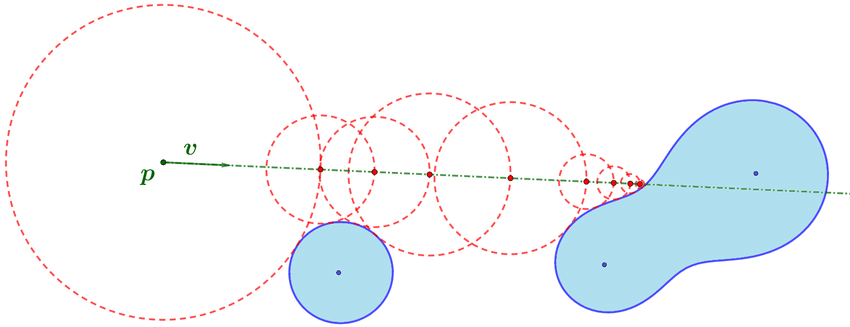
\includegraphics[width=0.6\textwidth]{sphere_tracing.png}
    \caption{Representación visual del algoritmo de sphere tracing, en el que cada círculo representa el rango libre de obstáculos determinado por la SDF.}
    \label{fig:sphere-tracing}
\end{figure}

\subsection{Ventajas y limitaciones de las SDF}

Las SDF ofrecen varias ventajas sobre los métodos de modelado tradicionales:

\begin{itemize}
    \item \textbf{Compacidad}: Las SDF se definen por fórmulas matemáticas en lugar de listas de vértices, lo que reduce el espacio necesario para describir objetos complejos.
    \item \textbf{Facilidad de combinación}: La geometría puede combinarse empleando operadores matemáticos (unión, intersección, resta) de forma eficiente y expresiva.
    \item \textbf{Transformaciones geométricas}: Las transformaciones como traslación, rotación y escalado se aplican directamente sobre la función, facilitando la manipulación.
    \item \textbf{Cálculo de normales}: La normal en la superficie se obtiene como el gradiente de la función de distancia, lo que simplifica el cálculo de iluminación.
    \item \textbf{Flexibilidad}: Permiten crear transiciones suaves entre objetos mediante operadores suavizados, lo que es difícil de lograr con mallas.
\end{itemize}

Pero también presentan diferentes limitaciones a la hora de representar geometría:

\begin{itemize}
    \item \textbf{Precision y aliasing}: El umbral de colisión y el número de pasos afectan la calidad de la imagen y pueden causar aliasing o superficies rugosas.
    \item \textbf{Superficies delgadas}: Si la SDF varía abruptamente o la superficie es muy fina, el avance óptimo se reduce y el número de pasos aumenta significativamente.
    \item \textbf{Efectos avanzados}: Efectos como la refracción y la reflexión requieren múltiples rayos y aumentan el coste computacional.
    \item \textbf{Desempeño}: El rendimiento depende de la complejidad de las funciones SDF y del número de objetos en escena.
\end{itemize}

\section{WebGPU: Acceso moderno a la GPU}

WebGPU es un estándar gráfico de nueva generación que proporciona acceso
eficiente y multiplataforma a la GPU, tanto en navegadores como en aplicaciones
nativas. Surge como respuesta a las limitaciones de APIs tradicionales
como OpenGL y DirectX, ofreciendo mayor control sobre el hardware, mejor
rendimiento y portabilidad.

\subsection{Motivación y principios de diseño}

WebGPU fue diseñado para proporcionar los siguientes atributos a los desarrolladores:

\begin{itemize}
    \item \textbf{Multiplataforma}: Disponible en Windows, Linux, macOS y en navegadores modernos (Chrome, Firefox, Safari).
    \item \textbf{Eficiencia}: Permite describir el flujo de datos entre la CPU y la GPU mediante buffers y pipelines, minimizando el coste de las llamadas de función y la sobrecarga del sistema.
    \item \textbf{Seguridad y portabilidad}: WebGPU abstrae detalles específicos del hardware, garantizando que el mismo código funcione en diferentes dispositivos y plataformas.
    \item \textbf{Modelo explícito}: El usuario configura directamente los recursos (buffers, texturas, pipelines) y controla el ciclo de vida de los datos, permitiendo optimizaciones avanzadas.
\end{itemize}

En contraste con OpenGL/WebGL, WebGPU obliga a definir explícitamente los
recursos y su uso, lo que mejora la seguridad y el rendimiento pero requiere
una mayor comprensión del modelo de GPU.

\subsection{Conceptos clave de WebGPU}

\begin{itemize}
    \item \textbf{Buffers}: Áreas de memoria para almacenar datos como vértices, índices y uniforms.
    \item \textbf{Textures}: Imágenes y mapas de datos que pueden ser leídos y escritos por la GPU.
    \item \textbf{Bind Groups}: Conjuntos de recursos que se vinculan a los shaders, permitiendo el acceso eficiente a datos en la GPU.
    \item \textbf{Pipelines}: Describen la secuencia de operaciones gráficas, incluyendo shaders, estados de rasterización y configuración de recursos.
    \item \textbf{Shaders}: Programas ejecutados en la GPU que transforman datos y calculan colores de píxeles.
    \item \textbf{Command Buffers}: Secuencias de instrucciones que la GPU ejecuta para renderizar o procesar datos.
\end{itemize}

WebGPU utiliza el lenguaje WGSL (\textit{WebGPU Shading Language}) para la
programación de shaders, ofreciendo una sintaxis moderna y expresiva adaptada a
las necesidades de la computación gráfica actual.

\section{Shaders y lenguaje WGSL}

Los \textbf{shaders} son programas que ejecutan operaciones matemáticas en la
GPU para transformar vértices, calcular colores y simular efectos visuales. En
WebGPU, los shaders se escriben en WGSL (\textit{WebGPU Shading Language}), un
lenguaje moderno diseñado para expresar funciones de distancia, operadores
booleanos, cálculos de iluminación y efectos visuales de forma eficiente.

\begin{itemize}
    \item \textbf{Vertex shaders}: Transforman posiciones y atributos de vértices.
    \item \textbf{Fragment shaders}: Calculan el color final de cada píxel, aplicando modelos de iluminación como Blinn-Phong, efectos de sombras y combinaciones de SDF.
\end{itemize}

WGSL permite aprovechar la arquitectura de la GPU para realizar renderizado en
tiempo real, combinando eficiencia y expresividad.

\subsection{Dawn: Implementación nativa de WebGPU}

\textbf{Dawn} es una implementación nativa de la API WebGPU desarrollada por Google y la comunidad Chromium\cite{dawn}. Dawn permite ejecutar aplicaciones que usan WebGPU fuera del navegador, proporcionando acceso directo y multiplataforma a la GPU. Es el backend utilizado por Copper para interactuar con WebGPU desde C++.

En Copper, Dawn se integra como una dependencia externa, permitiendo:

\begin{itemize}
    \item \textbf{Creación de instancias de WebGPU}: A través de las clases y funciones de Dawn, Copper inicializa \texttt{wgpu::Instance}, \texttt{wgpu::Device}, y otros objetos fundamentales.
    \item \textbf{Gestión de recursos}: Dawn facilita la creación y gestión de buffers, texturas y pipelines, siguiendo la especificación de WebGPU.
    \item \textbf{Integración con GLFW}: Mediante el módulo \texttt{webgpu-glfw}, Copper conecta la gestión de ventanas de GLFW con las superficies de renderizado de Dawn/WebGPU.
\end{itemize}

El ciclo de inicialización y renderizado en Copper se basa en la creación de la
instancia de Dawn (\texttt{CreateInstance}), la selección de adaptador y
dispositivo (\texttt{GetAdapter}, \texttt{GetDevice}), y la configuración de la
superficie de dibujo (\texttt{ConfigureSurface}). Los comandos de renderizado
se envían a la GPU mediante \texttt{CommandEncoder} y
\texttt{RenderPassEncoder}, siguiendo el modelo de WebGPU.

\section{Herramientas auxiliares}

El desarrollo de aplicaciones gráficas requiere gestionar ventanas, entrada de
usuario y la interfaz gráfica. Copper utiliza las siguientes herramientas:

\begin{itemize}
    \item \textbf{GLFW}: Biblioteca multiplataforma para la gestión de ventanas y eventos, usada a partir de su módulo de Dawn\cite{glfw-docs}.
    \item \textbf{ImGui}: Sistema de interfaz gráfica inmediata para la manipulación interactiva de primitivas y parámetros de escena\cite{imgui}.
    \item \textbf{GLM}: Biblioteca matemática para operaciones con vectores y matrices\cite{glm}.
    \item \textbf{CMake}: Herramienta de compilación y gestión de dependencias\cite{cmake-docs}.
\end{itemize}

Estas herramientas proporcionan la infraestructura básica para la interacción y
visualización dentro del entorno de Copper.
\chapter{Arquitectura del sistema y compilación}

El desarrollo de una aplicación gráfica interactiva como \textit{Copper}
requiere una base estructural robusta que garantice la separación de
responsabilidades, la mantenibilidad y la escalabilidad del código. Una
arquitectura de software bien definida es fundamental para gestionar la
complejidad inherente a la renderización en tiempo real, la gestión del estado
de la escena y la interacción con el usuario.

En este capítulo se presenta un análisis detallado de la arquitectura de
\textit{Copper}. El sistema no sigue de forma estricta ningún patrón de diseño,
sino que implementa una arquitectura por componentes con una fuerte
inspiración en el patrón Modelo-Vista-Controlador (MVC). Este enfoque
pragmático permite que cada componente se especialice en una tarea concreta
(renderizado, lógica de la escena, control de entrada), interactuando con otros
para construir la funcionalidad completa de la aplicación.

A continuación, se describirán los componentes principales, sus
responsabilidades y las interacciones entre ellos.

\section{Visión General de la Arquitectura}

La arquitectura de \textit{Copper} se puede descomponer en cuatro capas lógicas
principales que encapsulan las diferentes funcionalidades, como se ve en la
Figura\ref{fig:diagrama_arquitectura}.

\begin{figure}[H]
    \begin{center}
    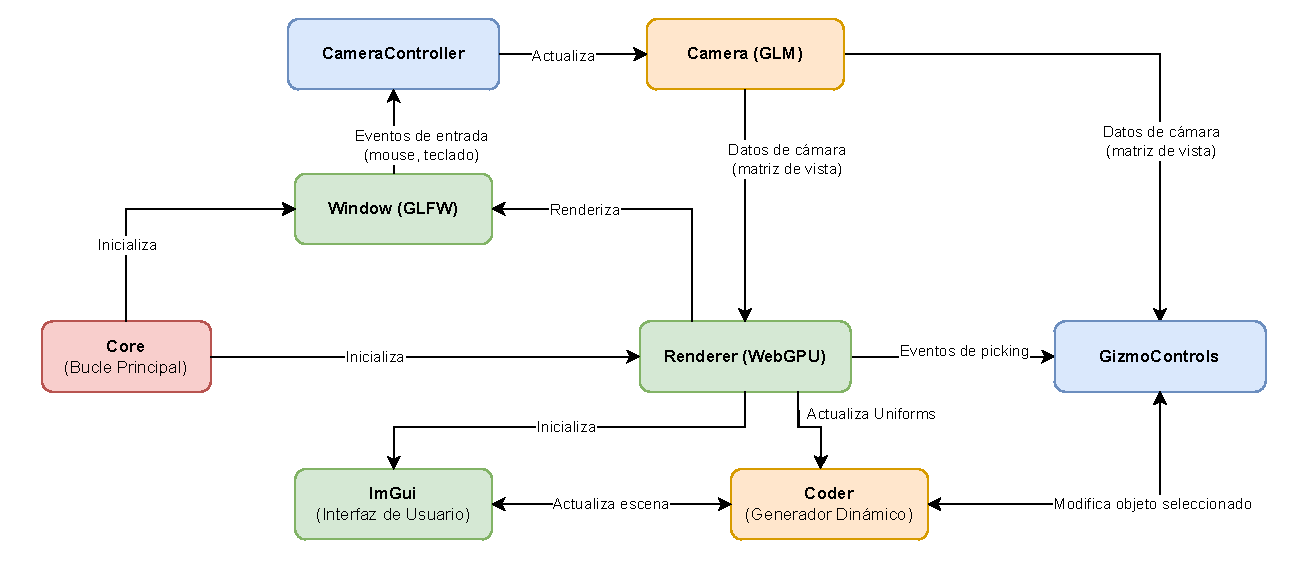
\includegraphics[width=0.95\textwidth]{imagenes/diagrama_arquitectura.pdf}
    \end{center}
    \caption{Diagrama de la arquitectura por componentes de \textit{Copper}.}
    \label{fig:diagrama_arquitectura}
\end{figure}

Las capas identificadas son:

\begin{itemize}
    \item \textbf{Capa de Orquestación y Ciclo de Vida (rojo):} Responsable de inicializar, ejecutar y terminar la aplicación. Es el punto de entrada y el gestor del bucle principal.
    \item \textbf{Capa de Datos y Lógica de la Escena (Modelo) (naranja):} Contiene el estado de la escena 3D, incluyendo los objetos, sus propiedades y la cámara. Encapsula la lógica de negocio, como la generación dinámica de shaders.
    \item \textbf{Capa de Presentación (Vista) (verde):} Se encarga de toda la representación visual, tanto el renderizado de la escena 3D mediante WebGPU como la interfaz gráfica de usuario (GUI) construida con ImGui.
    \item \textbf{Capa de Control de Usuario (Controlador) (azul):} Captura y procesa las entradas del usuario (ratón y teclado) y las traduce en acciones que modifican el estado del Modelo o la Vista.
\end{itemize}

Esta separación permite que, por ejemplo, se pueda modificar el motor de
renderizado (\texttt{Renderer}) sin afectar a la lógica de la escena
(\texttt{Coder}), o cambiar la forma en que se controla la cámara
(\texttt{CameraController}) sin alterar su representación de datos
(\texttt{Camera}).

\section{Análisis de Componentes por Capa}

A continuación, se detallan los componentes clave dentro de cada capa lógica,
referenciando sus ficheros de implementación.

\subsection{Capa de Orquestación y Ciclo de Vida}

El núcleo de la aplicación reside en la clase \texttt{Core}, definida en
\texttt{src/core/Core.h} y \texttt{src/core/Core.cpp}.

\begin{description}
    \item[\texttt{Core}:] Actúa como el orquestador principal. Su responsabilidad es inicializar todos los subsistemas en el orden correcto (\texttt{Core::Initialize}), gestionar el bucle principal de la aplicación (\texttt{Core::MainLoop}) y liberar los recursos de forma ordenada al finalizar (\texttt{Core::Terminate}). El bucle principal consulta el estado de la ventana y delega la tarea de dibujado al \texttt{Renderer} en cada fotograma.
\end{description}

\subsection{Capa de Datos y Lógica de la Escena (Modelo)}

Esta capa representa el estado y la lógica de negocio de la aplicación.

\begin{description}
    \item[\texttt{Coder} (\texttt{src/core/Coder.h}, \texttt{.cpp})]: Es el componente central del modelo. Gestiona la lista de objetos 3D de la escena (\texttt{std::vector<Object>}), sus propiedades (posición, color, forma) y las operaciones booleanas entre ellos. Su responsabilidad más crítica es el método \texttt{generateShaderCode()}, que traduce dinámicamente el estado de los objetos en código de shader WGSL. Este mecanismo es la "lógica de negocio" principal de \textit{Copper}, ya que define cómo se representa visualmente la escena. También se encarga de la persistencia de la escena mediante las funciones \texttt{saveScene()} y \texttt{loadScene()}.

    \item[\texttt{Camera} (\texttt{src/core/Camera.h}, \texttt{.cpp})]: Representa los datos y el estado de la cámara virtual. Almacena la matriz de vista (\texttt{view\_matrix}) y proporciona métodos para acceder a sus vectores fundamentales (posición, dirección, etc.). Aunque es una entidad pasiva, es una parte fundamental del modelo de datos, ya que define la perspectiva desde la que se observa la escena.
\end{description}

\subsection{Capa de Presentación (Vista)}

Esta capa es responsable de todo lo que el usuario ve en la pantalla.

\begin{description}
    \item[\texttt{Renderer} (\texttt{src/core/Renderer.h}, \texttt{.cpp})]: Es la vista principal. Su función es dibujar la escena 3D utilizando la API WebGPU. Orquesta el proceso de renderizado en su método \texttt{Render()}, donde toma los datos del \texttt{Coder} y la \texttt{Camera}, actualiza los \textit{uniforms} del shader y ejecuta los comandos de dibujado. También gestiona recursos de la GPU como la \textit{pipeline} de renderizado y los búferes.

    \item[\texttt{Interfaz} (\texttt{src/ui/Interfaz.h}, \texttt{.cpp})]: Componente especializado de la vista que gestiona la Interfaz Gráfica de Usuario (GUI) mediante la biblioteca ImGui. Es responsable de crear todos los paneles, botones y controles deslizantes que permiten al usuario interactuar con la aplicación. Lee el estado directamente del \texttt{Coder} para mostrar las propiedades de los objetos y, a su vez, invoca métodos en el \texttt{Coder} para modificar dicho estado, lo que representa una desviación del patrón MVC estricto.

    \item[\texttt{Window} (\texttt{src/ui/Window.h}, \texttt{.cpp})]: Gestiona la ventana nativa de la aplicación utilizando GLFW. Proporciona el "lienzo" sobre el que dibujan el \texttt{Renderer} y la \texttt{Interfaz}. Además, es responsable de registrar y despachar los eventos de entrada del sistema operativo (como clics de ratón o cambios de tamaño) a los componentes correspondientes.
\end{description}

\subsection{Capa de Control de Usuario (Controlador)}

Esta capa gestiona la entrada del usuario y la traduce en comandos para el
Modelo y la Vista.
\begin{description}
    \item[\texttt{CameraController} (\texttt{src/core/CameraController.h}, \texttt{.cpp})]: Es un controlador especializado en la manipulación de la cámara. Captura los eventos de arrastre del ratón y la rueda de desplazamiento para calcular la nueva orientación y posición de la cámara. En su método \texttt{update\_camera()}, modifica directamente el estado del objeto \texttt{Camera} (el Modelo) para reflejar la interacción del usuario.

    \item[\texttt{GizmoControls} (\texttt{src/core/GizmoControls.h}, \texttt{.cpp})]: Otro controlador altamente especializado, dedicado a la manipulación de los gizmos de transformación de los objetos. Cuando el usuario interactúa con un gizmo, esta clase calcula el desplazamiento correspondiente y actualiza la posición del objeto seleccionado. El nuevo estado se comunica al \texttt{Coder} para que la escena se actualice.

    \item[\texttt{Renderer} como despachador de eventos]: Excepcionalmente, la clase \texttt{Renderer} también asume un rol de controlador, debido al picking realizado por shader. Su método \texttt{OnMouseButton()} actúa como un punto de entrada que decide si la acción del usuario corresponde a una selección de objeto (lo que desencadena la pipeline de \textit{picking}) o a la manipulación de un gizmo (delegando el control a \texttt{GizmoControls}).
\end{description}

\section{Conclusiones sobre la Arquitectura}

La arquitectura de \textit{Copper} puede definirse como un sistema basado en
componentes con una clara separación de responsabilidades, que se alinea con
los principios del patrón Modelo-Vista-Controlador (MVC) sin seguir su
implementación más estricta.

La separación es evidente:
\begin{itemize}
    \item \textbf{Modelo}: \texttt{Coder} y \texttt{Camera} contienen el estado y la lógica central.
    \item \textbf{Vista}: \texttt{Renderer} e \texttt{Interfaz} se ocupan de la presentación visual.
    \item \textbf{Controlador}: \texttt{CameraController} y \texttt{GizmoControls} gestionan la entrada del usuario de forma aislada.
\end{itemize}

Sin embargo, se observan desviaciones pragmáticas del patrón MVC clásico, como
la comunicación directa entre la Vista (\texttt{Interfaz}) y el Modelo
(\texttt{Coder}) para modificar propiedades de objetos. Este enfoque, común en
aplicaciones gráficas, reduce la complejidad al eliminar la necesidad de un
controlador intermediario para cada pequeña modificación de estado.

En conclusión, la estructura elegida es eficaz y adecuada para una aplicación
de modelado 3D. Promueve la cohesión dentro de cada componente y mantiene un
bajo acoplamiento entre las distintas capas lógicas, lo que facilita el
mantenimiento, la depuración y la futura expansión del software.

\section{Sistema de construcción y compilación del proyecto}

El proyecto utiliza \textbf{CMake} como sistema de construcción para gestionar
la compilación, las dependencias y la organización de los archivos fuente.
CMake es una herramienta ampliamente empleada en proyectos de desarrollo de
software en C y C++ por su capacidad para generar archivos de construcción para
distintos sistemas y entornos \cite{cmake-docs}.

\subsection{Estructura del archivo CMake}

En la raíz del proyecto se encuentra el archivo \texttt{CMakeLists.txt}, que
define la configuración de la construcción. Sus principales componentes y
funcionalidades son:

\begin{itemize}
    \item \textbf{Definición del proyecto:}\\
          El proyecto se denomina \texttt{Copper}, está configurado para compilar en C++20 y se identifica como una aplicación de modelado 3D basada en SDF:
          \begin{lstlisting}[language=CMake, caption={Definición del proyecto en CMakeLists.txt}]
            project(Copper VERSION 0.0.2 LANGUAGES CXX C DESCRIPTION "3D SDF-based modeling application")
            set(CMAKE_CXX_STANDARD 20)
            set(CMAKE_CXX_STANDARD_REQUIRED ON)
            set(CMAKE_CXX_EXTENSIONS OFF)
\end{lstlisting}

    \item \textbf{Gestión de dependencias externas:}\\
          El archivo especifica la inclusión y compilación de bibliotecas externas necesarias para el funcionamiento del proyecto, como Dawn (WebGPU), GLM (matemáticas), ImGuiFileDialog (diálogos de archivos en la interfaz gráfica), y las fuentes de ImGui. La gestión de dependencias se realiza mediante \texttt{add\_subdirectory} y \texttt{FetchContent}, permitiendo su descarga y compilación automática junto al proyecto principal.
          Es importante el uso de \texttt{DAWN\_FETCH\_DEPENDENCIES} para no tener que instalar todas las librerías que usa Dawn ya que estos son pesados y pueden no ser necesarios, y así evitamos gestionar manualmente las dependencias.

    \item \textbf{Organización de los archivos fuente:}\\
          Se recopilan y organizan los archivos fuente del proyecto, excluyendo explícitamente el fichero \texttt{main.cpp} para evitar duplicidad, y se añaden los archivos fuente de ImGui.
          \begin{lstlisting}[language=CMake, caption={Organización de los archivos fuente en CMakeLists.txt}]
            file(GLOB_RECURSE COPPER_SOURCES src/*.cpp src/*.h)
            list(REMOVE_ITEM COPPER_SOURCES ${CMAKE_SOURCE_DIR}/src/main.cpp)\end{lstlisting}

    \item \textbf{Creación del ejecutable:}\\
          Se define el ejecutable principal \texttt{copper}, que se compila a partir de \texttt{main.cpp}, los archivos fuente propios y los de ImGui.
          \begin{lstlisting}[language=CMake, caption={Creación del ejecutable en CMakeLists.txt}]
    add_executable(copper src/main.cpp ${COPPER_SOURCES} ${IMGUI_SOURCES})\end{lstlisting}

    \item \textbf{Definición de directorios de inclusión:}\\
          Se especifican los directorios que contienen los archivos de cabecera para facilitar la compilación.
          \begin{lstlisting}[language=CMake, caption={Definición de directorios de inclusión en CMakeLists.txt}]
    target_include_directories(copper PRIVATE src lib/imgui lib/imgui/misc/cpp lib/imgui/backends ${CMAKE_CURRENT_BINARY_DIR}/src)\end{lstlisting}

    \item \textbf{Vinculación de bibliotecas:}\\
          Se vinculan las bibliotecas necesarias para el funcionamiento del programa, como Dawn/WebGPU, GLM, GLFW y el soporte para WebGPU en GLFW.
          \begin{lstlisting}[language=CMake, caption={Vinculación de bibliotecas en CMakeLists.txt}]
    target_link_libraries(copper PRIVATE dawn::webgpu_dawn glm::glm glfw webgpu_glfw ImGuiFileDialog)\end{lstlisting}

    \item \textbf{Definiciones de compilador:}\\
          Se incluyen definiciones específicas que permiten, por ejemplo, indicar el directorio de recursos y activar la integración de ImGui con WebGPU usando Dawn.
          \begin{lstlisting}[language=CMake, caption={Definiciones de compilador en CMakeLists.txt}]
                target_compile_definitions(copper PRIVATE RESOURCE_DIR="${CMAKE_CURRENT_SOURCE_DIR}/src" IMGUI_IMPL_WEBGPU_BACKEND_DAWN)
\end{lstlisting}
\end{itemize}

\subsection{Proceso de compilación}

El desarrollo principal se ha llevado a cabo sobre un entorno Linux, aunque la
elección de herramientas y librerías multiplataforma debería asegurar su compilación en
otros sistemas operativos como Windows o macOS, esto podría requerir ajustes en
la configuración del proyecto.

Para compilar el proyecto, se debe disponer de CMake y un compilador compatible
con C++20. El proceso estándar usando git para compilar el proyecto consiste
en:

\begin{enumerate}
    \item Si fuese necesario añadir los paquetes utilizados por Dawn:
          \begin{lstlisting}[language=bash]
        sudo apt-get install libxrandr-dev libxinerama-dev libxcursor-dev mesa-common-dev libx11-xcb-dev pkg-config nodejs npm\end{lstlisting}
    \item Clonar el repositorio de Git y actualizar los submódulos:
          \begin{lstlisting}[language=bash]
        git clone https://github.com/tu-usuario/copper.git
        cd copper
        git submodule update --init\end{lstlisting}
    \item Compilar en la carpeta build:
          \begin{lstlisting}[language=bash]
        cmake -B build
        cmake --build build -j$(nproc)\end{lstlisting}
    \item Por último si se quiere ejecutar el proyecto:
          \begin{lstlisting}[language=bash]
        ./build/copper\end{lstlisting}
\end{enumerate}

Esto construirá el ejecutable \texttt{copper}, incluyendo todas las
dependencias y archivos fuente indicados en \texttt{CMakeLists.txt}.

\subsection{Función del sistema de construcción}

El sistema CMake facilita:

\begin{itemize}
    \item La gestión automática de dependencias externas.
    \item La configuración multiplataforma.
    \item La compilación eficiente de todos los módulos del programa, asegurando que las
          dependencias y rutas de inclusión están correctamente resueltas.
    \item La integración de recursos y librerías de terceros necesarios para la ejecución
          (por ejemplo, ImGui para la interfaz gráfica, Dawn para el acceso a WebGPU).
\end{itemize}

La configuración descrita en el archivo \texttt{CMakeLists.txt} permite
reproducir el proceso de compilación en distintos sistemas, facilitando el
trabajo colaborativo y la portabilidad del proyecto.
\chapter{Implementación del módulo Ventana}

\section{Introducción}

El módulo \textbf{Ventana} constituye el punto de entrada visual y de
interacción para el sistema. Este componente es responsable de la
creación, gestión y destrucción de la ventana principal de la aplicación, así
como del manejo de eventos de usuario y del ciclo de vida asociado a la
interfaz gráfica.

\section{Diseño y estructura de la clase Window}

La clase \texttt{Window}, ubicada en \texttt{src/ui/Window.h} y
\texttt{src/ui/Window.cpp}, encapsula toda la funcionalidad relacionada con la
ventana.

\subsection{Atributos principales}

\begin{itemize}
    \item \texttt{GLFWwindow* window}: Puntero al objeto de ventana gestionado por GLFW.
    \item \texttt{uint32\_t windowWidth, windowHeight}: Dimensiones internas de la ventana, actualizadas dinámicamente.
\end{itemize}

\subsection{Métodos públicos}

\begin{itemize}
    \item \texttt{bool Initialize(Renderer *renderer)}: Inicializa la ventana, configurando parámetros gráficos y de interacción, y registra los callbacks de eventos. La ventana se crea con una relación de aspecto fija (16:9), facilitando la integración con el pipeline gráfico y evitando distorsiones.
    \item \texttt{GLFWwindow* getWindow()}: Permite acceder al objeto de ventana desde otros módulos, especialmente el \texttt{Renderer} y la interfaz gráfica.
    \item \texttt{uint32\_t getWindowWidth()}, \texttt{getWindowHeight()}: Proporcionan las dimensiones actuales, utilizadas en la configuración de la proyección y el cálculo del aspecto.
    \item \texttt{void setWindowSize(uint32\_t width, uint32\_t height)}: Permite modificar las dimensiones internas de la ventana, útil en escenarios de redimensionado.
    \item \texttt{void Destroy()}: Libera los recursos asociados a la ventana, llamando a \texttt{glfwDestroyWindow}.
    \item \texttt{void SetWindowUserPointer(void* pointer)}: Permite asociar un puntero de usuario (normalmente, el \texttt{Renderer}) para su acceso desde los callbacks de eventos.
\end{itemize}

\subsection{Callbacks de eventos}

La clase Window define y registra varios callbacks estáticos:

\begin{itemize}
    \item \texttt{FramebufferSizeCallback(GLFWwindow* window, int width, int height)}: Se ejecuta cuando la ventana es redimensionada. Utiliza el puntero de usuario para acceder al \texttt{Renderer} y llama a su método \texttt{OnResize()}, lo que desencadena la reconfiguración de los buffers gráficos y la superficie de renderizado. Esto garantiza que el aspecto visual de la escena se mantenga correcto ante cualquier cambio de tamaño.
    \item \texttt{MouseButtonCallback(GLFWwindow *window, int button, int action, int mods)}: Captura los eventos de pulsación de botones de ratón. Si la interfaz gráfica (ImGui) no está capturando el ratón, el evento se propaga al método \texttt{OnMouseButton} del \texttt{Renderer}, permitiendo la interacción directa con los objetos 3D a partir de los gizmos.
\end{itemize}

El registro de los callbacks se realiza en el método \texttt{Initialize},
asegurando que todos los eventos relevantes sean gestionados desde el inicio de
la aplicación.

\section{Proceso de inicialización y configuración}

El proceso de inicialización de la ventana sigue una secuencia de pasos bien
definida:

\begin{enumerate}
    \item Llamada a \texttt{glfwInit()} para inicializar la biblioteca GLFW.
    \item Configuración de los hints de ventana (\texttt{GLFW\_CLIENT\_API},
          \texttt{GLFW\_RESIZABLE}) para deshabilitar la API gráfica por defecto y
          permitir el redimensionado.
    \item Obtención del monitor y modo de vídeo principal para adaptar la ventana al
          entorno gráfico del usuario.
    \item Creación de la ventana con \texttt{glfwCreateWindow}, ajustando el tamaño al
          modo de vídeo y estableciendo el título (\texttt{"Copper"}).
    \item Fijación de la relación de aspecto mediante \texttt{glfwSetWindowAspectRatio},
          asegurando que la escena 3D se muestre correctamente.
    \item Registro de los callbacks de eventos (\texttt{FramebufferSizeCallback},
          \texttt{MouseButtonCallback}).
    \item Configuración de los modos de entrada (\texttt{GLFW\_CURSOR},
          \texttt{GLFW\_RAW\_MOUSE\_MOTION}) para gestionar el cursor y la interacción
          avanzada.
\end{enumerate}

Este diseño asegura que la ventana esté lista para recibir eventos y para
integrarse con el sistema de renderizado desde el primer momento.

\section{Gestión avanzada de eventos}

El manejo de eventos en la ventana es fundamental para la interactividad del
sistema. El diseño implementado permite:

\begin{itemize}
    \item \textbf{Sincronización con el pipeline gráfico}: Los eventos de redimensionado se propagan automáticamente al \texttt{Renderer}, que actualiza buffers, superficie y matrices de proyección, manteniendo la coherencia visual.
    \item \textbf{Integración con ImGui}: Antes de procesar eventos de ratón, se comprueba si ImGui está capturando el ratón, evitando conflictos entre la interfaz gráfica y la manipulación 3D.
    \item \textbf{Extensibilidad}: Aunque el callback de movimiento de ratón (\texttt{MouseMoveCallback}) está declarado, no se encuentra activado por defecto, permitiendo su futura ampliación sin modificar la estructura principal.
\end{itemize}

El siguiente fragmento de código muestra la gestión y propagación de eventos
(\texttt{Window.cpp}):

\begin{verbatim}
void Window::MouseButtonCallback(GLFWwindow *window, int button, int action, int mods) {
    auto* renderer = static_cast<Renderer*>(glfwGetWindowUserPointer(window));
    if (renderer != nullptr && !ImGui::GetIO().WantCaptureMouse) {
        renderer->OnMouseButton(button, action);
    }
}
\end{verbatim}

\section{Interacción con el ciclo de vida de la aplicación}

La ventana se integra en el ciclo de vida de la aplicación a través del módulo
\texttt{Core} (\texttt{src/core/Core.cpp}, \texttt{src/core/Core.h}), que
gestiona su inicialización y destrucción. El flujo es el siguiente:

\begin{enumerate}
    \item \texttt{Core::Initialize()} llama a \texttt{window.Initialize(&renderer)} y a \texttt{renderer.Init(&window)}, asegurando que la ventana y el sistema gráfico están listos antes de iniciar el bucle principal.
    \item Durante la ejecución, \texttt{Core::MainLoop()} llama a
          \texttt{glfwPollEvents()} y a \texttt{renderer.Render()}, manteniendo la
          actualización continua de la ventana y la escena.
    \item Al finalizar, \texttt{Core::Terminate()} invoca \texttt{window.Destroy()} y
          \texttt{glfwTerminate()}, liberando todos los recursos y evitando fugas de
          memoria.
\end{enumerate}

\section{Decisiones técnicas y justificación}

La elección de GLFW como biblioteca para la gestión de ventanas se justifica
por varios motivos:

\begin{itemize}
    \item \textbf{Portabilidad}: GLFW es multiplataforma, permitiendo ejecutar Copper en diferentes sistemas operativos sin cambios en el código.
    \item \textbf{Compatibilidad}: La integración con WebGPU y con ImGui está ampliamente soportada, simplificando el desarrollo y la depuración.
    \item \textbf{Modularidad}: El diseño de la clase \texttt{Window} permite modificar el backend de ventanas sin afectar al resto del sistema, siguiendo el principio de separación de responsabilidades.
    \item \textbf{Eficiencia}: La gestión nativa de eventos y la actualización dinámica de los buffers gráficos optimizan el rendimiento y la fluidez de la aplicación.
\end{itemize}

Estas decisiones están alineadas con las recomendaciones de la literatura
técnica (Sommerville, 2016) y con las guías docentes de la ETSIIT, que
aconsejan implementar componentes modulares, eficientes y fácilmente
mantenibles.

\section{Interacción con otros componentes}

El módulo Ventana está estrechamente integrado con:

\begin{itemize}
    \item \texttt{Renderer}: Recibe y procesa los eventos relevantes para actualizar el pipeline gráfico y la escena.
    \item \texttt{Interfaz gráfica (GUI)}: Sirve como base para la integración de ImGui, permitiendo la edición y visualización de parámetros y objetos.
    \item \texttt{Subsistema de cámara y controles}: Los eventos de entrada capturados por la ventana se transmiten al controlador de cámara y gizmos, facilitando la manipulación interactiva de la escena.
\end{itemize}

La arquitectura facilita la extensión futura del sistema, permitiendo añadir
nuevas funcionalidades (por ejemplo, soporte para pantallas múltiples o
diferentes sistemas de entrada) sin modificar la lógica principal.

\section{Flujo de datos y ciclo de vida}

Durante la ejecución de la aplicación, la ventana realiza las siguientes
tareas:

\begin{itemize}
    \item Recoge eventos de entrada (ratón, teclado, redimensionado) y los distribuye
          entre los módulos correspondientes.
    \item Mantiene actualizadas las dimensiones de la ventana, permitiendo al renderer
          ajustar el aspecto y las matrices de proyección.
    \item Facilita la integración de la interfaz gráfica y la visualización de los
          controles de usuario.
\end{itemize}

El ciclo de vida completo está gestionado por el módulo \texttt{Core},
garantizando la correcta inicialización y liberación de recursos.

\chapter{Implementación de la cámara}

Las cámaras son un componente esencial en cualquier sistema de renderizado 3D,
ya que permiten definir el punto de vista desde el que se observa la escena. En
Copper, la cámara está implementada a través de las clases \texttt{Camera} y
\texttt{CameraController}, las cuales gestionan tanto la transformación de la
vista como la interacción del usuario. A continuación, se describe
detalladamente cómo se representa y utiliza la cámara en Copper, desde la
construcción de la matriz de vista hasta su uso en los shaders mediante el
sistema de \texttt{Uniforms}.

\section{La matriz de vista en Copper}

En Copper, la cámara se representa principalmente mediante una matriz de vista
(\texttt{view\_matrix}), que transforma las coordenadas de los objetos del
espacio de mundo al espacio de la cámara. La clase \texttt{Camera} mantiene la
posición del ojo (\texttt{eye}), el punto de interés (\texttt{center}), y el
vector de orientación vertical (\texttt{up}), que se usan para construir la
matriz de vista.

\begin{equation}
    \bm{V}
    =
    \begin{pmatrix}
        \vec{x}_x & \vec{x}_y & \vec{x}_z & c_x
        \\
        \vec{y}_x & \vec{y}_y & \vec{y}_z & c_y
        \\
        \vec{z}_x & \vec{z}_y & \vec{z}_z & c_z
        \\
        0         & 0         & 0         & 1
    \end{pmatrix}.
\end{equation}

Aquí, $\vec{\bm{x}}$, $\vec{\bm{y}}$ y $\vec{\bm{z}}$ son los vectores base del
espacio de la cámara, y $\vec{\bm{c}}$ es la posición de la cámara. Los
vectores base son vectores unitarios que definen la orientación de la cámara;
son ortogonales entre sí. Los vectores $\vec{\bm{x}}$, $\vec{\bm{y}}$ y
$\vec{\bm{z}}$ también se conocen como los vectores derecho, arriba y adelante
respectivamente. El vector hacia adelante siempre apunta en la dirección en la
que la cámara está mirando. En la \ref{fig:camera_view_matrix_vectors_diagram}
se muestra un diagrama de la vista de la cámara, que muestra cómo están
orientados los vectores base en el espacio. La posición de la cámara
$\vec{\bm{c}}$ es la posición de la cámara, en coordenadas de cámara.

\begin{figure} [!hbt]
    \begin{center}
        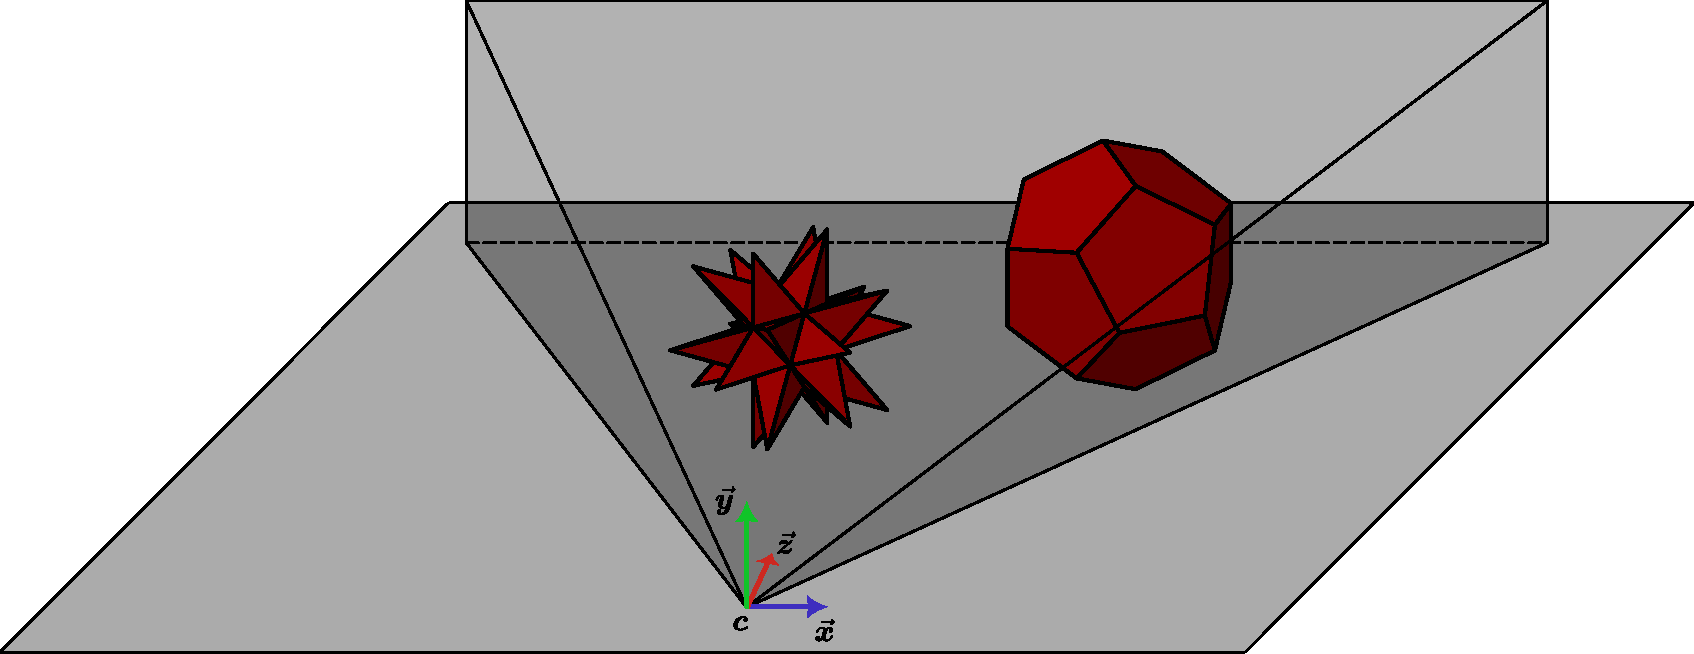
\includegraphics[width=0.95\textwidth]{imagenes/view_matrix_vectors_diagram.pdf}
    \end{center}
    \caption{Vectores base del espacio de la cámara, $\vec{\bm{x}}$, $\vec{\bm{y}}$, $\vec{\bm{z}}$ y posición $\bm{c}$.}\label{fig:camera_view_matrix_vectors_diagram}
\end{figure}

La matriz de vista se actualiza usando la función \texttt{glm::lookAt} de la
biblioteca GLM:

\begin{lstlisting}[language=C++,caption={Actualización de la matriz de vista en Copper}]
void Camera::update_view_matrix() {
    this->view_matrix = glm::lookAt(
        this->eye,
        this->center,
        this->up
    );
}
\end{lstlisting}

Esta función genera una matriz de 4x4 que realiza una traslación y rotación
para situar el origen de coordenadas en la posición de la cámara y orientar los
ejes de acuerdo a los vectores especificados. Los métodos
\texttt{get\_right()}, \texttt{get\_up()} y \texttt{get\_forward()} permiten
obtener los vectores base del espacio de la cámara directamente desde la matriz
de vista transpuesta.

\section{Control de la cámara y actualización de la vista}

La clase \texttt{CameraController} gestiona la interacción del usuario para
modificar la vista de la cámara mediante el ratón y el scroll, permitiendo
rotar, trasladar y acercar/alejar la cámara respecto al centro de la escena. El
controlador calcula la nueva orientación usando cuaterniones y actualiza la
matriz de vista de la cámara en función de los movimientos del usuario.

\begin{lstlisting}[language=C++,caption={Actualización de la vista desde CameraController}]
void CameraController::update_view_matrix() {
    auto matrix = glm::transpose(
        mat4_cast(this->total_rotation)
    );

    auto right = glm::vec3(matrix[0]);
    auto up = glm::vec3(matrix[1]);
    auto view_dir = glm::vec3(matrix[2]);

    auto camera_center = this->center;
    auto translation = glm::vec3(
        glm::dot(right, camera_center),
        glm::dot(up, camera_center),
        glm::dot(view_dir, camera_center));

    matrix[0][3] = translation.x;
    matrix[1][3] = translation.y;
    matrix[2][3] = translation.z - this->radius;

    this->camera->set_view_matrix(glm::transpose(matrix));
}
\end{lstlisting}

\section{Paso de la matriz de cámara al shader: Uniforms}

Para que el shader pueda utilizar la información de la cámara, la matriz de
vista se pasa como parte de la estructura \texttt{Uniforms}. En Copper, antes
de cada renderizado, la matriz de vista se actualiza y se copia a los datos de
\texttt{uniformsData}, que luego se transfieren a la GPU:

\begin{lstlisting}[language=C++,caption={Actualización del uniform con la matriz de vista}]
uniformsData.mvp_matrix = this->camera->get_view_matrix();
device.GetQueue().WriteBuffer(uniformsBuffer, 0, &uniformsData, sizeof(Uniforms));
\end{lstlisting}

En el shader (WGSL), se accede a esta matriz a través del binding de
\texttt{Uniforms}:

\begin{lstlisting}[language=C++,caption={Uso de la matriz de cámara en el shader}]
struct Uniforms {
    mvp_matrix: mat4x4<f32>,
    //...
};
@group(0) @binding(0) var<uniform> uniforms: Uniforms;

@fragment
fn fragmentMain(in: VertexOutput) -> @location(0) vec4<f32> {
    let cam = transpose(uniforms.mvp_matrix);
    let right = cam[0].xyz;
    let up = cam[1].xyz;
    let forward = cam[2].xyz;
    let eye = cam[0].w * right + cam[1].w * up + cam[2].w * forward;
    //...
}
\end{lstlisting}

La operación \texttt{transpose(uniforms.mvp\_matrix)} permite extraer los
vectores principales de la cámara desde la matriz de vista, siguiendo la
convención de OpenGL y GLM. \break

\subsection{Motivos para utilizar una matriz $4\times4$ en la cámara de Copper}

Aunque el cálculo de los rayos de visión en Copper se realiza utilizando
únicamente los vectores principales de la cámara (derecha, arriba y adelante),
es decir, operando esencialmente en tres dimensiones, la matriz de cámara
(\texttt{view\_matrix}) se mantiene en formato $4\times4$ durante todo el
pipeline, a pesar de poder simplificarse a una matriz $3\times4$. Esta decisión se ha tomado por razones de compatibilidad,
flexibilidad y coherencia con las convenciones de las principales APIs y
bibliotecas gráficas.

La matriz de proyección tradicional en gráficos 3D requiere el uso de coordenadas homogéneas ($x, y, z, w$) y
matrices $4\times4$ para poder representar la perspectiva correctamente\cite{Ahn2008}. Sin
embargo, en Copper, no se aplica una matriz de proyección, si no que el cálculo de la perspectiva se
realiza directamente en el shader, utilizando únicamente los vectores de la
cámara y los parámetros de \texttt{aspect\_ratio} y \texttt{FOV}.

En resumen, \textbf{Copper calcula la perspectiva y el ray tracing únicamente
    en tres dimensiones, pero mantiene la matriz de cámara en formato $4\times4$
    por compatibilidad, facilidad de desarrollo y flexibilidad futura}. Este diseño
permite adaptar el sistema a cambios sin necesidad de reescribir partes
significativas del código y sigue las convenciones del desarrollo gráfico
moderno.

\chapter{Implementación de los Shaders}

\section{Introducción}

En este capítulo se describe la implementación de los shaders en el sistema
Copper, explicando cómo se genera el código shader, su funcionamiento, y el
proceso mediante el cual se parametriza y escribe el código según la escena y
los objetos definidos por el usuario.

\section{Arquitectura General}

Copper utiliza renderizado basado en shaders escritos en WGSL (WebGPU Shading
Language), generando el código de manera dinámica a partir de la descripción de
la escena. La clase principal responsable de esta tarea es \texttt{Coder}, que
compone el código shader en tiempo de ejecución según los objetos y operaciones
definidos.

\section{Funcionamiento General}

El ciclo de generación y uso de shaders sigue el siguiente flujo:

\begin{enumerate}
    \item El usuario define objetos geométricos (esferas, cajas, conos, cilindros) y
          operaciones booleanas (unión, intersección, sustracción suave, etc.) a través
          de la interfaz gráfica.
    \item Cada vez que la escena cambia, la clase \texttt{Coder} reconstruye el código
          shader combinando funciones SDF (Signed Distance Function) para cada objeto y
          operación.
    \item El código generado incluye la lógica para renderizado normal y picking
          (selección de objetos).
    \item El shader se compila y se utiliza en la pipeline gráfica de WebGPU.
\end{enumerate}

\section{Generación Dinámica del Código Shader}

La clase \texttt{Coder} mantiene una lista de objetos y sus propiedades (tipo,
posición, tamaño, color, operación). Cuando la escena cambia, el método
\texttt{generateShaderCode()} produce el código WGSL correspondiente. El
proceso es el siguiente:

\begin{itemize}
    \item Para cada objeto, se genera una función SDF específica que calcula la distancia
          y el color.
    \item Se combinan las SDFs utilizando las operaciones booleanas indicadas (por
          ejemplo, unión suave, intersección, sustracción).
    \item Se añade lógica para picking, de modo que cada objeto pueda ser seleccionado
          mediante raycasting.
    \item Si hay objetos auxiliares como gizmos, se añaden funciones SDF para estos
          elementos.
    \item El código generado se concatena junto con una base estándar que define la
          estructura de los shaders, funciones de iluminación, ray marching, etc.
\end{itemize}

\section{Ejemplo de Código Generado}

El siguiente fragmento ilustra parte del código shader que se puede generar
dinámicamente:

\begin{lstlisting}[language=C++, caption={Fragmento de código WGSL generado}]
fn sdf(pos: vec3<f32>) -> DistanceColor {
    var result = DistanceColor(1e6, vec3<f32>(0.0, 0.0, 0.0), -1);
    var sphere0: DistanceColor = sdf_sphere(pos, uniforms.position, uniforms.size[0], uniforms.color, 0);
    result = opSmoothUnion(result, sphere0, 0.6);
    // ... otros objetos y operaciones
    return result;
}
\end{lstlisting}

\section{Personalización y Parametrización}

La generación del shader se adapta a los parámetros definidos por el usuario:

\begin{itemize}
    \item \textbf{Parámetros geométricos}: posición, tamaño y color de cada objeto se insertan directamente en el código WGSL.
    \item \textbf{Operaciones}: el tipo de operación (unión, intersección, sustracción suave) determina qué función de combinación se utiliza.
    \item \textbf{Picking}: se genera una función especial que permite identificar qué objeto ha sido seleccionado por el usuario.
    \item \textbf{Gizmos}: si el usuario selecciona un objeto, se generan SDFs adicionales para los gizmos de manipulación.
\end{itemize}

\section{Funciones SDF y Operaciones Booleanas}

Cada tipo de objeto tiene su propia función SDF:

\begin{itemize}
    \item \texttt{sdf\_sphere}: calcula la distancia de un punto al borde de una esfera.
    \item \texttt{sdf\_box}: calcula la distancia a una caja.
    \item \texttt{sdf\_cone}, \texttt{sdf\_cylinder}: para conos y cilindros.
    \item \texttt{sdf\_plane}: para planos.
\end{itemize}

Las combinaciones entre objetos se realizan con operadores booleanos suaves:

\begin{lstlisting}[language=C++, caption={Operadores booleanos suaves}]
fn opSmoothUnion(d1: DistanceColor, d2: DistanceColor, k: f32) -> DistanceColor { ... }
fn opSmoothIntersect(d1: DistanceColor, d2: DistanceColor, k: f32) -> DistanceColor { ... }
fn opSmoothSubtract(d1: DistanceColor, d2: DistanceColor, k: f32) -> DistanceColor { ... }
\end{lstlisting}

\section{Renderizado y Ray Marching}

El shader utiliza ray marching para recorrer la escena y determinar la
superficie más cercana en cada píxel. Para cada paso:

\begin{itemize}
    \item Se evalúa la función SDF combinada para todos los objetos.
    \item Al encontrar una superficie (distancia menor a un umbral), se calcula el color
          aplicando iluminación tipo Blinn-Phong.
    \item Se calcula el sombreado y las normales mediante diferencias finitas.
\end{itemize}

\section{Picking en el shader}

La técnica de \textbf{picking} en Copper permite identificar el objeto SDF
seleccionado por el usuario, usando un shader especializado que recorre la
escena y devuelve el identificador (\texttt{id}) del objeto más próximo al rayo
lanzado desde el cursor.

El proceso es el siguiente:

\begin{enumerate}
    \item Al pulsar el botón izquierdo del ratón, se genera una pipeline de picking y se
          ejecuta el shader picking.
    \item En el shader, se calcula el rayo a partir de la posición del cursor,
          transformada a coordenadas normalizadas y ajustada por la matriz de vista de
          cámara.
    \item Se realiza ray marching sobre la escena, evaluando la función SDF y almacenando
          el \texttt{id} del objeto más cercano.
    \item El resultado se escribe en un buffer (generalmente una textura de un solo canal
          entero), que se lee desde la CPU para determinar el objeto seleccionado.
\end{enumerate}

El núcleo del shader de picking, generado dinámicamente por la clase
\texttt{Coder}, se parece a este fragmento:

\begin{lstlisting}[language=C++, caption={Picking shader fragment}]
@fragment
fn fragmentPickingMain(in: VertexOutput) -> @location(0) i32{
    let cam = transpose(uniforms.mvp_matrix);
    let right = cam[0].xyz;
    let up = cam[1].xyz;
    let forward = cam[2].xyz;
    let eye = cam[0].w * right + cam[1].w * up + cam[2].w * forward;
    let m = uniforms.mouse_position * 2.0 - vec2<f32>(1.0, 1.0);
    let mouse_uv = vec2<f32>(m.x, -m.y / uniforms.aspect_ratio);
    let rd = normalize(mouse_uv.x * right + mouse_uv.y * up + FOV * forward);
    let ro = eye;
    let dc = ray_march_picking(ro, rd);
    return dc.id;
}
\end{lstlisting}

La función \texttt{ray\_march\_picking} recorre la escena utilizando la función
SDF de picking, que para cada objeto evalúa la distancia y el identificador:

\begin{lstlisting}[language=C++, caption={Ray marching picking loop}]
fn ray_march_picking(ro: vec3<f32>, rd: vec3<f32>) -> DistanceColor {
    var total_distance: f32 = 0.0;
    for (var i: i32 = 0; i < MAX_MARCHING_STEPS && total_distance < MAX_DISTANCE; i++) {
        let pos = ro + rd * total_distance;
        let dc = sdf_picking(pos);
        if (dc.distance < MIN_DISTANCE) {
            return dc;
        }
        total_distance += dc.distance;
    }
    return DistanceColor(1e6, vec3<f32>(0.0), -1);
}
\end{lstlisting}

La función \texttt{sdf\_picking} está generada dinámicamente y recorre todos
los objetos, devolviendo el identificador del más cercano:

\begin{lstlisting}[language=C++, caption={SDF picking para todos los objetos}]
fn sdf_picking(pos: vec3<f32>) -> DistanceColor {
    var result = DistanceColor(1e6, vec3<f32>(0.0, 0.0, 0.0), -1);
    // Para cada objeto:
    // var sphere0: DistanceColor = sdf_sphere(...);
    // ...
    if (sphere0.distance < result.distance) {
        result = sphere0;
    }
    // ...
    return result;
}
\end{lstlisting}

El pipeline de picking escribe el \texttt{id} del objeto seleccionado en la
textura de picking, que luego es leída por la CPU para actualizar el estado de
selección en el sistema.

\chapter{Implementación y diseño de los controles}

\section{Introducción}

El sistema de controles en Copper permite la manipulación de la escena 3D y la
interacción directa con los objetos SDF (Signed Distance Fields). Este capítulo
describe en profundidad la arquitectura, matemáticas y tecnologías utilizadas,
y se divide en dos apartados: controles de interfaz gráfica (ImGui) y controles
de gizmo (GizmoControls).

\begin{figure}[H]
	\centering
	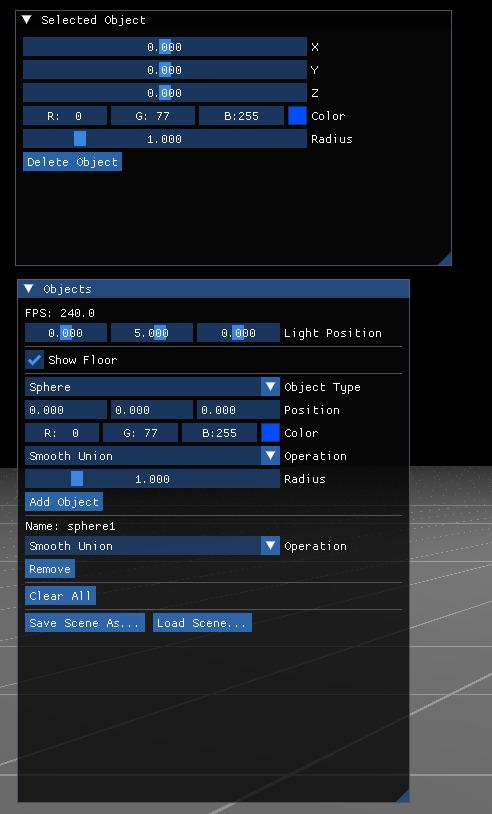
\includegraphics[width=0.7\textwidth]{imagenes/ImGui.jpg}
	\caption{Interfaz gráfica basada en ImGui.}
\end{figure}

\section{Controles de interfaz gráfica: ImGui}

El módulo de interfaz gráfica (\texttt{Interfaz.cpp}, \texttt{Interfaz.h})
utiliza \textbf{ImGui} para implementar menús, sliders y herramientas de
edición.

\subsection{Estructura y funciones principales}

La clase \texttt{Interfaz} interactúa con los módulos \texttt{Coder} y
\texttt{Renderer} para:
\begin{itemize}
    \item Mostrar propiedades de objetos seleccionados (posición, color, tipo, tamaño).
    \item Permitir la edición directa mediante sliders y campos de entrada.
    \item Gestionar la creación, edición y borrado de objetos SDF.
    \item Proporcionar controles globales de la escena (luz, renderizado, operaciones).
    \item Implementar la gestión de archivos para guardar y cargar escenas.
\end{itemize}

\subsection{Ejemplo de interacción}

Al seleccionar un objeto, ImGui presenta sus propiedades y permite
modificarlas:
\begin{lstlisting}[language=C++,caption={Edición de propiedades de un objeto SDF seleccionado}]
ImGui::SliderFloat("X", &selectedObject.x, -10.0f, 10.0f);
ImGui::ColorEdit3("Color", &selectedObject.r);
// Para esferas:
ImGui::SliderFloat("Radius", &selectedObject.size[0], 0.1f, 5.0f);
\end{lstlisting}
Cada cambio marca el pipeline como "dirty" para que el renderizador actualice
la escena en tiempo real.

\section{Controles de gizmo: GizmoControls}

El módulo \texttt{GizmoControls} (\texttt{GizmoControls.cpp},
\texttt{GizmoControls.h}) permite la manipulación visual e interactiva de los
objetos SDF seleccionados mediante gizmos (flechas, planos).

\begin{figure}[H]
	\centering
	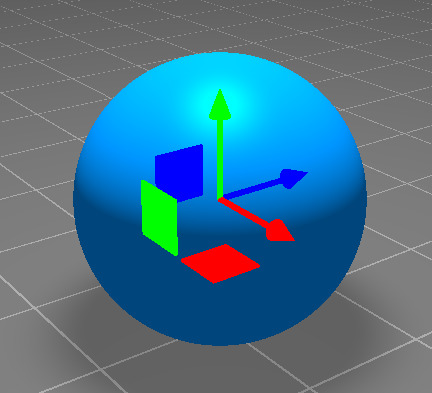
\includegraphics[width=0.7\textwidth]{imagenes/gizmo.jpg}
	\caption{Visualización de gizmo de manipulación.}
\end{figure}

\subsection{Arquitectura y flujo de interacción}

\begin{itemize}
    \item \textbf{Inicialización}: Al seleccionar un objeto y pulsar sobre el gizmo, se inicia la manipulación (\texttt{initDrag}).
    \item \textbf{Picking}: Se determina qué parte del gizmo ha sido seleccionada (eje, plano) usando ray marching y cálculos de distancia mínimos.
    \item \textbf{Arrastre y movimiento}: El punto de intersección inicial se calcula con \texttt{gizmoIntersection} y se actualiza en tiempo real mientras el usuario mueve el ratón.
    \item \textbf{Actualización de propiedades}: El centro del objeto se actualiza en \texttt{update}, propagando el nuevo valor al objeto seleccionado en el módulo \texttt{Coder}.
\end{itemize}


\subsection{Gizmo de movimiento lineal en ejes X, Y y Z}

Para implementar el gizmo de movimiento lineal, es necesario implementar un
sistema que detecte la cantidad de movimiento en cada eje con respecto al
desplazamiento del ratón. Esto significa transformar unas coordenadas
\textit{screen space} (2D) a coordenadas \textit{world space} (3D).

El sistema implementado se basa en la intersección entre dos líneas en
\text{world space}, una línea que representa al eje sobre el que queremos mover
el objeto, y otra línea, que representa el rayo \textit{casteado} desde la
posición del ratón. Este último rayo parte de la posición de la cámara y se
extiende hacia el plano de la escena. La sección de \textit{raymarching}
explica como transformar una coordenada UV de la pantalla a rayos casteados
desde la posición de la cámara.

Como en 3D es difícil hacer que dos líneas se crucen, y la precisión perdida en
las aproximaciones de coma flotante podría afectar a los cálculos. Hemos
decidido utilizar una expresión para el punto más cercano entre dos líneas.
Estas expresiones son ampliamente conocidas y se puede encontrar en múltiples
fuentes. A continuación se deja un desarrollo propio.

Sean dos líneas en el espacio 3D, definidas por sus ecuaciones paramétricas:

\begin{equation}
    \begin{cases}
        p_1 = k_1 + l_1  \vec{v}_1, \\
        p_2 = k_2 + l_2  \vec{v}_2.
    \end{cases}
\end{equation}

Dónde $k_1$ y $k_2$ son dos puntos por los que pasan las líneas, $\vec{v}_1$ y
$\vec{v}_2$ son sus vectores directores, y $l_1$ y $l_2$ son los parámetros que
recorren las líneas, dos números reales. La distancia entre dos puntos
arbitrarios en cada línea, $p_1$ y $p_2$, se puede expresar como:

\begin{equation}
    d = \| p_1 - p_2 \| = \| (k_1 + l_1 * \vec{v}_1) - (k_2 + l_2 * \vec{v}_2) \|.
\end{equation}

Descomponiendo los vectores y puntos en sus componentes y tomando el cuadrado
de la distancia, obtenemos:

\begin{equation}
    \begin{align}
        d^2 = & \left(k_{1_x} + l_1 v_{1_x} - k_{2_x} - l_2 v_{2_x}\right)^2  \\
        +     & \left(k_{1_y} + l_1 v_{1_y} - k_{2_y} - l_2 v_{2_y}\right)^2  \\
        +     & \left(k_{1_z} + l_1 v_{1_z} - k_{2_z} - l_2 v_{2_z}\right)^2.
    \end{align}
\end{equation}

Teniendo en cuenta que solo tenemos dos variables, ambas al cuadrado, podemos
ver que \(d^2\) es una parábola tridimensional. Como la parábola es positiva,
todos los puntos están por encima de $d = 0$, solo tiene un mínimo, el mínimo
global. Nuestro problema tiene por tanto una sola solución, que podemos
encontrar buscando este mínimo, (no tendremos que descartar puntos de silla).

El mínimo lo encontraremos en el punto en el que la derivada de $d^2$ con
respecto a $l_1$ y $l_2$ sea cero.

\begin{align}
     & \begin{align}
           \frac{\partial d^2}{\partial l_1} = 0 = 2\left(k_{1_x} + l_1 v_{1_x} - k_{2_x} - l_2 v_{2_x}\right)v_{1_x} \\
           + 2\left(k_{1_y} + l_1 v_{1_y} - k_{2_y} - l_2 v_{2_y}\right)v_{1_y}                                       \\
           + 2\left(k_{1_z} + l_1 v_{1_z} - k_{2_z} - l_2 v_{2_z}\right)v_{1_z},
       \end{align}  \\
     & \begin{align}
           \frac{\partial d^2}{\partial l_2} = 0 = -2\left(k_{1_x} + l_1 v_{1_x} - k_{2_x} - l_2 v_{2_x}\right)v_{2_x} \\
           -2\left(k_{1_y} + l_1 v_{1_y} - k_{2_y} - l_2 v_{2_y}\right)v_{2_y}                                         \\
           + 2\left(k_{1_z} + l_1 v_{1_z} - k_{2_z} - l_2 v_{2_z}\right)v_{2_z}.
       \end{align}
\end{align}
Desarrollando estas ecuaciones podemos obtener:

\begin{align}
    l1 & = \frac{l_2 \vec{v}_2\cdot\vec{v}_2 - k_1\cdot k_2 + k_2\cdot k_2 } { v_1\cdot v_2},                                                                                                                                                                               \\
    l2 & = \frac{\frac{\vec{v}_1\cdot{\vec{v}_1}}{\vec{v}_1\cdot\vec{v}_2}(k_2\cdot\vec{v}_2 - k_1\cdot\vec{v}_2) + k_1\cdot \vec{v}_1 - k_2\cdot\vec{v}_1}{\vec{v}_1\cdot\vec{v}_2 - \frac{(\vec{v}_2\cdot\vec{v}_2) (\vec{v}_1\cdot\vec{v}_1)}{\vec{v}_1\cdot\vec{v}_2}},
\end{align}
los parámetros que debemos introducir en las ecuaciones paramétricas de las líneas para obtener los puntos más cercanos entre ambas.

\subsection{Gizmo de movimiento en planos XY, XZ y YZ}

El movimiento en un plano del gizmo (por ejemplo, el plano XY) utiliza un
enfoque geométrico distinto al del movimiento lineal. En lugar de encontrar la
distancia mínima entre dos líneas, el sistema calcula la intersección directa
entre el rayo del ratón y el plano de movimiento.

El proceso, implementado en las funciones \texttt{GizmoControls::update} y
\texttt{gizmoIntersection}, es el siguiente:

\begin{enumerate}
    \item \textbf{Definición del plano}: Cuando se selecciona un gizmo de plano (por ejemplo, el plano XY), el sistema lo define mediante un punto que contiene (el centro del objeto, \texttt{objectCenter}) y su vector normal. Es importante destacar que, por convención en el código, el vector almacenado en \texttt{currentGizmo} para un plano es su normal. Por ejemplo, para el plano XY, la normal es el eje Z (0, 0, 1).
    \item \textbf{Intersección Rayo-Plano}: Con cada movimiento del ratón, se vuelve a castear un rayo desde la cámara (\texttt{ro}, \texttt{rd}). La función \texttt{planeLineIntersection} calcula el punto exacto donde este rayo intersecta el plano infinito definido en el paso anterior. La ecuación para la intersección de una línea y un plano es una fórmula geométrica estándar.
    \item \textbf{Cálculo del Desplazamiento}: El sistema calcula el vector de desplazamiento (\texttt{diffV}) restando el punto de intersección inicial (\texttt{firstIntersectionPoint}, calculado en \texttt{initDrag}) del punto de intersección actual.
          \begin{verbatim}
glm::vec3 diffV = intersection - this->firstIntersectionPoint;
    \end{verbatim}
    \item \textbf{Aplicación del Movimiento Restringido}: El desplazamiento \texttt{diffV} se suma a la posición inicial del objeto (\texttt{initialObjectCenter}) para obtener la nueva posición teórica. Sin embargo, para asegurar que el objeto solo se mueva en el plano seleccionado, se aplica una máscara vectorial. Esta máscara se crea restando el vector normal del plano al vector identidad \texttt{glm::vec3(1.0)}.
          \begin{itemize}
              \item Para el plano XY, la normal es (0, 0, 1). La máscara es (1, 1, 1) - (0, 0, 1) =
                    (1, 1, 0).
              \item Para el plano XZ, la normal es (0, 1, 0). La máscara es (1, 1, 1) - (0, 1, 0) =
                    (1, 0, 1).
              \item Para el plano YZ, la normal es (1, 0, 0). La máscara es (1, 1, 1) - (1, 0, 0) =
                    (0, 1, 1).
          \end{itemize}
          Al multiplicar la nueva posición por esta máscara, se anula cualquier movimiento en la dirección de la normal, restringiendo el desplazamiento exclusivamente al plano deseado.
\end{enumerate}

Este método garantiza que, aunque el ratón se mueva en un espacio 2D y el rayo
viaje en 3D, el objeto seleccionado se deslice perfectamente sobre el plano
elegido, proporcionando un control intuitivo y preciso.
\chapter{Funcionalidades adicionales implementadas}

\section{Introducción}

Además de las capacidades principales de modelado y renderizado SDF, Copper
incorpora un conjunto de funcionalidades adicionales que mejoran la experiencia
de usuario, la usabilidad y la flexibilidad del sistema. En este capítulo se
describen y documentan con detalle las funcionalidades que han sido añadidas
sobre la base del código existente y su integración en los distintos módulos.

\section{Gestión de la escena: guardado y carga}

La posibilidad de guardar y cargar escenas permite al usuario almacenar el
estado actual del modelado y recuperarlo posteriormente. Esta funcionalidad
está implementada en el módulo \texttt{Coder}, mediante los métodos
\texttt{saveScene} y \texttt{loadScene} (\texttt{src/core/Coder.cpp},
\texttt{src/core/Coder.h}).
\subsection{Guardar escena}

El método \texttt{saveScene(const std::string\& filename)} serializa todos los
objetos presentes en la escena, incluyendo tipo, posición, tamaño, color,
operación y el identificador único. El formato del archivo es texto plano y
sigue una estructura legible, facilitando la interoperabilidad y la depuración.

\subsection{Cargar escena}

El método \texttt{loadScene(const std::string\& filename)} permite restaurar la
escena a partir de un archivo previamente guardado. El sistema parsea cada
línea, reconstruye los objetos y actualiza su identificador, asegurando la
coherencia y la compatibilidad con versiones futuras.

\subsection{Integración en la interfaz}

La gestión de archivos está directamente integrada en la interfaz gráfica
(\texttt{src/ui/Interfaz.cpp}), mediante el uso de \texttt{ImGuiFileDialog}. El
usuario puede seleccionar el archivo deseado para guardar o cargar la escena, y
el sistema actualiza la visualización en tiempo real. Este flujo está soportado
por el siguiente fragmento:

\begin{verbatim}
if (ImGuiFileDialog::Instance()->IsOk()) {
    std::string filePath = ImGuiFileDialog::Instance()->GetFilePathName();
    coder->saveScene(filePath);
}
\end{verbatim}


\section{Visualización de FPS y métricas}

La interfaz muestra el número de frames por segundo (FPS) utilizando
\texttt{ImGui::GetIO().Framerate}, permitiendo valorar el rendimiento del
sistema durante la edición y el renderizado.

\chapter{Conclusiones y mejoras futuras}

En este documento se ha presentado el sistema Copper, un entorno de desarrollo
para la creación y manipulación de escenas 3D basadas en Signed Distance Fields
(SDF). A lo largo de los capítulos, se ha detallado la arquitectura,
implementación y funcionamiento de sus principales componentes, incluyendo la
gestión de controles, la implementación de shaders y el sistema de picking.

Entre las conclusiones más relevantes, se destacan las siguientes:

\begin{itemize}
      \item La utilización de SDF permite una representación eficiente y flexible de la
            geometría 3D, facilitando operaciones complejas como la unión, intersección y
            sustracción de objetos.
      \item La integración de herramientas de interfaz gráfica (ImGui) y gizmos proporciona
            una experiencia de usuario intuitiva y directa para la manipulación de la
            escena.
      \item El sistema de picking implementado permite seleccionar objetos de manera
            precisa, incluso en escenas complejas, mejorando la interactividad del entorno.
\end{itemize}

En cuanto a mejoras futuras, se proponen las siguientes líneas de trabajo:

\begin{itemize}
      \item Ampliación de las capacidades de edición en tiempo real, permitiendo a los
            usuarios modificar más propiedades y mayor variedad de objetos.
      \item Implementación de un sistema de materiales y texturas más avanzado, que permita
            una mejor representación visual de los objetos en la escena.
      \item Mejora del sistema de renderizado, optimizando el uso de la GPU y añadiendo
            mejoras como el antialiasing.
      \item Estudiar la portabilidad del sistema a web, debido a la elección de tecnologías
            como WebGPU es un área de desarrollo evidente.
      \item Añadir un sistema de exportación de la escena a formatos de malla estándar
            (como OBJ o GLTF) para facilitar la interoperabilidad con otras herramientas y
            flujos de trabajo. Con este objetivo, se ha estudiado la aplicación del
            algoritmo Marching Cubes, que permite convertir las representaciones basadas en
            SDF a mallas poligonales compatibles con estos formatos.
\end{itemize}

Estas mejoras contribuirán a consolidar a Copper como una herramienta potente y
versátil para la creación de escenas 3D, ampliando sus posibilidades y
mejorando la experiencia del usuario.


%
\nocite{*}
\addcontentsline{toc}{chapter}{Bibliografía}
\bibliographystyle{miunsrturl}
\printbibliography
%
\appendix
\chapter{Código}
\chapter{Escenas}

\newglossaryentry{nombre en pdf}{
name={Nombre definicion},
description={definicion}
}

\glsaddall
\addcontentsline{toc}{chapter}{Glosario}
\printglossaries
\chapter*{}
\thispagestyle{empty}

\end{document}